% This is "sig-alternate.tex" V2.1 April 2013
% This file should be compiled with V2.5 of "sig-alternate.cls" May 2012
%
% This example file demonstrates the use of the 'sig-alternate.cls'
% V2.5 LaTeX2e document class file. It is for those submitting
% articles to ACM Conference Proceedings WHO DO NOT WISH TO
% STRICTLY ADHERE TO THE SIGS (PUBS-BOARD-ENDORSED) STYLE.
% The 'sig-alternate.cls' file will produce a similar-looking,
% albeit, 'tighter' paper resulting in, invariably, fewer pages.
%
% ----------------------------------------------------------------------------------------------------------------
% This .tex file (and associated .cls V2.5) produces:
%       1) The Permission Statement
%       2) The Conference (location) Info information
%       3) The Copyright Line with ACM data
%       4) NO page numbers
%
% as against the acm_proc_article-sp.cls file which
% DOES NOT produce 1) thru' 3) above.
%
% Using 'sig-alternate.cls' you have control, however, from within
% the source .tex file, over both the CopyrightYear
% (defaulted to 200X) and the ACM Copyright Data
% (defaulted to X-XXXXX-XX-X/XX/XX).
% e.g.
% \CopyrightYear{2007} will cause 2007 to appear in the copyright line.
% \crdata{0-12345-67-8/90/12} will cause 0-12345-67-8/90/12 to appear in the copyright line.
%
% ---------------------------------------------------------------------------------------------------------------
% This .tex source is an example which *does* use
% the .bib file (from which the .bbl file % is produced).
% REMEMBER HOWEVER: After having produced the .bbl file,
% and prior to final submission, you *NEED* to 'insert'
% your .bbl file into your source .tex file so as to provide
% ONE 'self-contained' source file.
%
% ================= IF YOU HAVE QUESTIONS =======================
% Questions regarding the SIGS styles, SIGS policies and
% procedures, Conferences etc. should be sent to
% Adrienne Griscti (griscti@acm.org)
%
% Technical questions _only_ to
% Gerald Murray (murray@hq.acm.org)
% ===============================================================
%
% For tracking purposes - this is V2.0 - May 2012

\documentclass{sig-alternate-05-2015}
% Maintain images and tables within their respective sections
\usepackage{caption} 

\graphicspath{ {images/} }

\def\sharedaffiliation{%
\end{tabular}
\begin{tabular}{c}}

\begin{document}

% Copyright
\setcopyright{acmcopyright}
%\setcopyright{acmlicensed}
%\setcopyright{rightsretained}
%\setcopyright{usgov}
%\setcopyright{usgovmixed}
%\setcopyright{cagov}
%\setcopyright{cagovmixed}

% DOI
\doi{10.475/123_4}

% ISBN
\isbn{123-4567-24-567/08/06}

%Conference
\conferenceinfo{ACSAC '16}{June 16--19, 2013, Seattle, WA, USA}

\acmPrice{\$15.00}

%
% --- Author Metadata here ---
\conferenceinfo{ACSAC}{'16 El Paso, Texas USA}
\CopyrightYear{2016} % Allows default copyright year (20XX) to be over-ridden - IF NEED BE.
%\crdata{0-12345-67-8/90/01}  % Allows default copyright data (0-89791-88-6/97/05) to be over-ridden - IF NEED BE.
% --- End of Author Metadata ---

\title{SuperTLS: A Diverse and Redundant Secure Communication Channel for Privacy in Cloud}
%\subtitle{[Extended Abstract]
%\titlenote{A full version of this paper is available as
%\textit{Author's Guide to Preparing ACM SIG Proceedings Using
%\LaTeX$2_\epsilon$\ and BibTeX} at
%\texttt{www.acm.org/eaddress.htm}}}
%
% You need the command \numberofauthors to handle the 'placement
% and alignment' of the authors beneath the title.
%
% For aesthetic reasons, we recommend 'three authors at a time'
% i.e. three 'name/affiliation blocks' be placed beneath the title.
%
% NOTE: You are NOT restricted in how many 'rows' of
% "name/affiliations" may appear. We just ask that you restrict
% the number of 'columns' to three.
%
% Because of the available 'opening page real-estate'
% we ask you to refrain from putting more than six authors
% (two rows with three columns) beneath the article title.
% More than six makes the first-page appear very cluttered indeed.
%
% Use the \alignauthor commands to handle the names
% and affiliations for an 'aesthetic maximum' of six authors.
% Add names, affiliations, addresses for
% the seventh etc. author(s) as the argument for the
% \additionalauthors command.
% These 'additional authors' will be output/set for you
% without further effort on your part as the last section in
% the body of your article BEFORE References or any Appendices.

\numberofauthors{3} %  in this sample file, there are a *total*
% of EIGHT authors. SIX appear on the 'first-page' (for formatting
% reasons) and the remaining two appear in the \additionalauthors section.
%
\author{
% You can go ahead and credit any number of authors here,
% e.g. one 'row of three' or two rows (consisting of one row of three
% and a second row of one, two or three).
%
% The command \alignauthor (no curly braces needed) should
% precede each author name, affiliation/snail-mail address and
% e-mail address. Additionally, tag each line of
% affiliation/address with \affaddr, and tag the
% e-mail address with \email.
%
% 1st. author
\alignauthor
Andr\'e Joaquim\\
       \affaddr{INESC-ID, Instituto Superior T\'ecnico, Universidade de Lisboa}\\
       \affaddr{Lisbon, Portugal}\\
% 2nd. author
\alignauthor
Miguel L. Pardal\\
       \affaddr{INESC-ID, Instituto Superior T\'ecnico, Universidade de Lisboa}\\
       \affaddr{Lisbon, Portugal}\\
% 3rd. author
\alignauthor
Miguel Correia\\
       \affaddr{INESC-ID, Instituto Superior T\'ecnico, Universidade de Lisboa}\\
       \affaddr{Lisbon, Portugal}\\
       %
       \end{tabular}
       \begin{tabular}{c}
       \email{\{andre.joaquim, miguel.pardal, miguel.p.correia\}@tecnico.ulisboa.pt}  
}
% use '\and' if you need 'another row' of author names
% There's nothing stopping you putting the seventh, eighth, etc.
% author on the opening page (as the 'third row') but we ask,
% for aesthetic reasons that you place these 'additional authors'
% in the \additional authors block, viz.
%\additionalauthors{Additional authors: John Smith (The Th{\o}rv{\"a}ld Group,
%email: {\texttt{jsmith@affiliation.org}}) and Julius P.~Kumquat
%(The Kumquat Consortium, email: {\texttt{jpkumquat@consortium.net}}).}
\date{03 May 2016}
% Just remember to make sure that the TOTAL number of authors
% is the number that will appear on the first page PLUS the
% number that will appear in the \additionalauthors section.

\maketitle
\begin{abstract}
We present SuperTLS, a diverse and redundant vulnerability-tolerant secure communication channel for privacy in cloud.
There have always been concerns about the strength of some of encryption mechanisms used in SSL/TLS channels and some of them were regarded as insecure at some point in time.
SuperTLS is our solution to mitigate the problem of secure communication channels being vulnerable to attacks due to unexpected vulnerabilities in its encryption mechanisms. It is based on diversity and redundancy of cryptographic mechanisms and certificates to provide a secure communication channel even when one or more mechanisms are regarded vulnerable.
SuperTLS relies on a combination of $k$ mechanisms/cipher suites, with $k$ being the diversity factor and $k > 1$.
Even when $k - 1$ mechanisms are regarded as insecure or considered vulnerable, SuperTLS relies on the remaining secure, diverse and redundant mechanism to maintain the channel secure.
We evaluated the performance of our channel by comparing it to a normal TLS channel.
\end{abstract}

%
% The code below should be generated by the tool at
% http://dl.acm.org/ccs.cfm
% Please copy and paste the code instead of the example below. 
%
\begin{CCSXML}
<ccs2012>
<concept>
<concept_id>10003033.10003039.10003051</concept_id>
<concept_desc>Networks~Application layer protocols</concept_desc>
<concept_significance>500</concept_significance>
</concept>
<concept>
<concept_id>10003033.10003083.10003014</concept_id>
<concept_desc>Networks~Network security</concept_desc>
<concept_significance>300</concept_significance>
</concept>
<concept>
<concept_id>10010520.10010575.10010755</concept_id>
<concept_desc>Computer systems organization~Redundancy</concept_desc>
<concept_significance>500</concept_significance>
</concept>
<concept>
<concept_id>10002978.10003014.10003015</concept_id>
<concept_desc>Security and privacy~Security protocols</concept_desc>
<concept_significance>300</concept_significance>
</concept>
<concept>
<concept_id>10002978.10002979.10002982</concept_id>
<concept_desc>Security and privacy~Symmetric cryptography and hash functions</concept_desc>
<concept_significance>100</concept_significance>
</concept>
</ccs2012>
\end{CCSXML}

\ccsdesc[500]{Networks~Application layer protocols}
\ccsdesc[300]{Networks~Network security}
\ccsdesc[500]{Computer systems organization~Redundancy}
\ccsdesc[300]{Security and privacy~Security protocols}
\ccsdesc[100]{Security and privacy~Symmetric cryptography and hash functions}

%
% End generated code
%

%
%  Use this command to print the description
%
\printccsdesc

\keywords{Secure communication channels; Diversity; Redundancy; TLS; Vulnerability-Tolerance}

\section{Introduction}

\textit{Secure communication channels} are mechanisms that allow two entities to exchange messages or information securely in the Internet.
A secure communication channel has three properties: \textit{authenticity}, \textit{confidentiality}, and \textit{integrity}. Regarding authenticity, in an authentic channel, the messages can not be tampered. Regarding confidentiality, in a confidential channel, only the original receiver of a message is able to read that message. Regarding integrity, no one can impersonate another. The information regarding the original sender of a message can not be changed.
Several secure communication channels exist nowadays, such as TLS, IPsec or SSH. Each of these examples is used for a different purpose, but with the same finality of securing the communication.

\textit{Transport Layer Security (TLS)} is a secure communication channel widely used. Originally called Secure Sockets Layer (SSL), its first released version was SSL 2.0, released in 1995. SSL 3.0 was released in 1996, bringing improvements to its predecessor such as allowing forward secrecy and supporting SHA-1.
Defined in 1999, TLS did not introduce major changes. Although, the changes introduced were enough to make TLS 1.0 incompatible with SSL 3.0.
% In order to grant compatibility, a TLS 1.0 connection can be downgraded to SSL 3.0, which brought security issues.
TLS 1.1 and TLS 1.2 are upgrades to TLS 1.0 which brought some improvements such as mitigating CBC (cipher block chaining) attacks and supporting more block cipher modes of operation to use with AES.
TLS is divided in two sub-protocols, Handshake and Record, constituted by several mechanisms each.
The Handshake protocol is used to establish or re-establish a communication between a server and client. The Record protocol is used to process the sent and received messages.

\textit{Internet Protocol Security (IPsec)} is an Internet layer protocol that protects the communication at a lower level than SSL/TLS, which operates at the Application layer \cite{IPsec}.

\textit{Secure Shell (SSH)} is an Application layer protocol, such as SSL/TLS. SSH is a protocol used for secure remote login and other secure network services over an insecure network \cite{SSH}.

A secure communication channel becomes insecure when a vulnerability is discovered. Vulnerabilities may concern the protocol's specification, cryptographic mechanisms used by the protocol or specific implementations of the protocol. Many vulnerabilities have been discovered in SSL/TLS originating new versions of the protocol with renewed security aspects such as deprecating cryptographic mechanisms or enforcing security measures.
Concrete implementations of SSL/TLS have been also considered vulnerable by having implementation details causing a breach of security and affecting devices worldwide.

SuperTLS is a secure communication channel tolerant to vulnerabilities which does not rely on only one cryptographic mechanism. It is our belief that \textit{diversity} and \textit{redundancy} of cryptographic mechanisms and certificates can help mitigate existent vulnerabilities.
In our project's context, diversity and redundancy consist in using two or more different mechanisms/cipher suites with the same objective. For example, MD5 and SHA-3 are both hash functions used to generate digests. In a real case, where MD5 has become insecure, our diverse and redundant secure communication channel relies upon SHA-3 to keep the communication secure. Using diversity and redundancy of cryptographic mechanisms, when a one of those mechanisms is successfully attacked, another mechanism is able to maintain the security and availability of the communication.

%\begin{itemize}
%	\item Maybe talk a little about the project's context -- the cloud and communication between clouds
%\end{itemize}

Using diversity and redundancy, SuperTLS aims at increasing security over current secure communication channels by guaranteeing a diversity factor $k > 1$, which implies having $k$ different cipher suites with optimally $k$ different mechanisms for key exchange, authentication, encryption and signing.

Although SSL/TLS supporting strong encryption mechanisms, such as AES and RSA, there are other factors than mathematical complexity that can contribute to vulnerabilities.
Diversifying encryption mechanisms includes diversifying certificates and consequently keys (public, private, shared).
Diversity of certificates is a direct consequence of diversifying encryption mechanisms due to the fact that each certificate is related to an authentication and key exchange mechanism.

The contributions of this paper are a new secure communication channel which uses diversity and redundancy to tolerate vulnerabilities in existent cryptographic mechanisms based on TLS 1.2 and specific evidence that diversity and redundancy can be employed without creating an excessive overhead in the communication. Proving that diversity and redundancy have a real impact on increasing security of a communication channel, while having reasonable performance and time-related costs, required a precise evaluation of our solution.

The rest of the document is organized in the following way: Section 2 presents the related work. Section 3 presents the architecture of the proposed solution. Section 4 presents the evaluation. Section 5 presents some conclusions.

\section{Related Work}
\label{sec-related-work}

Research was made in order to find previous studies about diversity, how encryption mechanisms can be combined and recent known attacks to secure communication channels, namely SSL/TLS. This section describes research done in these areas.

\subsection{Diversity in security}

Nowadays, one of the main security concerns is a system being static. A static system is a system where there are no changes with time. It is clear that a static system, or sitting-target, is more prone to attacks than a diverse system because, in static systems, an attacker has time to study the system's architecture and vulnerabilities.
This way, an attacker can perform several distinct attacks while the system remains the same.

On the opposite side, a diverse system is a system that changes with time.
The term \textit{diversity} describes multi-version software in which redundant versions are deliberately made different from one another \cite{Littlewood2004}.
Without diversity, there is just one program spread across devices around the world. Every device has the same program version, with the same vulnerabilities. Using diversity, we can present the attacker with modified programs, each one with modifications. There is no proper way of knowing the attacks which that particular program is susceptible to.

Software diversity targets mostly implementation details and the ability of the attacker to replicate the user's environment. Diversity does not change the program's logic. Therefore, diversity will not be helpful if a program is badly implemented.

\subsection{SSL/TLS Protocol}

A secure communication channel is a channel used by two entities to communicate with each other. A secure communication channel grants confidentiality and authenticity. Confidentiality is defined as keeping information secret. When Alice sends a message to Bob, only Bob can read that message. Confidentiality ensures that no one else will be able to read the message. Authenticity is defined as keeping information authentic. Authenticity ensures that no one tampered the message. Integrity is defined as keeping information honest. Integrity ensures that no one sends a message pretending to be someone else.

\subsubsection{The TLS Protocol}

The TLS protocol has two main sub-protocols -- the TLS Handshake Protocol and the TLS Record Protocol.

The TLS Handshake Protocol is a protocol used to establish or resume a secure session between two communicating parties -- a client and a server.
A session is established in several steps, each one corresponding to a different message:

\begin{enumerate}

\item {The client sends a \textit{ClientHello} message to the server. This message is sent when the client wants to connect to a server or as a response to a \textit{HelloRequest} from a server. The \textit{ClientHello} message is composed by the client's TLS version, a structure denominated \textit{Random}(which has a secure random number with 28 bytes and the current date and time), the session identifier, a list of the cryptographic mechanisms supported by the client and a list of compression methods supported by the client, both lists ordered by preference. The client may also request additional functionalities from the server.}

\item {The server responds with a \textit{ServerHello} message. The \textit{ServerHello} message is composed by the server's TLS version, a structure denominated \textit{Random} analogous to \textit{ClientHello}'s structure with the same name, the session identifier, a cryptographic mechanism and a compression method, both of them chosen by the server from the lists received in the \textit{ClientHello} message, and a list of extensions.}

\item {If the key exchange algorithm agreed between client and server requires authentication, the server sends its certificate to the client -- a \textit{Certificate} message.}

\item {A \textit{ServerKeyExchange} message is sent to the client after the \textit{Certificate} message if the server's certificate does not contain enough information in order to allow the client to share a premaster secret.}

\item {The server then sends a request for the client's certificate -- \textit{CertificateRequest}. This message is composed by a list of types of certificate the client may send, a list of the server's supported signature algorithms and a list of certificate authorities accepted by the server.}

\item {The server sends a \textit{ServerHelloDone} message to conclude his first sequence of messages.}

\item {After receiving the \textit{ServerHelloDone} message, the client sends its certificate to the server, if requested. When the server receives the client's certificate, there are some aspects that may risk the handshake. If the client does not send its certificate or if its certificate does not meet the server's conditions, the server may choose to continue or to abort the handshake.}

\item {The client proceeds to send to the server a \textit{ClientKeyExchange} message containing an encrypted premaster secret. The client generates a premaster secret with 48 bytes and encrypts it with the server's certificate public key. At this point, the server and the client use the premaster secret to generate the session keys and the master secret.}

\item {If the client's certificate possesses signing capability, a \textit{CertificateVerify} message is sent to the server. Its purpose is to explicitly verify the client's certificate.}

\item {The client must send a \textit{ChangeCipherSpec} message to the server. A \textit{ChangeCipherSpec} message is used to inform the server that the client is now using the agreed-upon algorithms for encryption and hashing. TLS has a specific protocol to signal transitions in ciphering strategies denominated Change Cipher Spec. According to this protocol, a \textit{ChangeCipherSpec} message must be sent by both client and server to notify one another that they are now using the algorithms agreed-upon.}

\item {The client now sends his last handshake message -- \textit{Finished}. The Finished message verifies the success of the key exchange and the authentication.}

\item {After receiving the \textit{ChangeCipherSpec} message, the server starts using the algorithms established previously and sends a \textit{ChangeCipherSpec} message to the client as well.}

\item {The server puts an end to the handshake protocol by sending a \textit{Finished} message to the client.}

\end{enumerate}

By this point, the session is established. Client and server can now exchange information (application data) through the secure communication channel.

The TLS Record protocol is the sub-protocol which processes the messages to be sent and the received ones.

Regarding an outgoing message, the first operation performed by the TLS Record protocol is fragmentation. The message is divided into blocks called TLSPlaintext. Each block contains the protocol version, the content type, the fragment of application data and this fragment's length in bytes. The fragment's length must be $2^{14}$ bytes or less.

After fragmenting the message, each block may be optionally compressed, using the compression method defined in the Handshake. 
The compression operation transforms each TLSPlaintext block into a TLSCompressed block. Each TLSCompressed block also contains the protocol version and content type as TLSPlaintext block and contains the compressed form of the fragment and its length. The fragment's length must be $2^{14} + 1024$ bytes or less.
Although there is always an active compression algorithm, the default algorithm is CompressionMethod.null. CompressionMethod.null is an operation that does nothing, i.e., no fields are altered. In this case, the TLSCompressed blocks are identical to the TLSPlaintext blocks and no changes are made.

Each TLSCompressed block is now transformed into a TLSCiphertext block by encryption and MAC functions. Each TLSCiphertext block contains the protocol version, content type and the encrypted form of the compressed fragment of application data, with the MAC, and the fragment's length.  The fragment's length must be $2^{14} + 2048$ bytes or less. When using block ciphers, it is also added a padding and its length to the block. The padding is added in order to force the length of the fragment to be a multiple of the block cipher's block length. When using AEAD ciphers, no MAC key is used.
The message is now sent to its destination.

Regarding an incoming message, the process is the inverse of the process for outgoing messages. The message is, therefore, decrypted, verified, decompressed, reassembled and delivered to the application.

\subsubsection{TLS vulnerabilities}
\label{tls-vulnerabilities}

TLS vulnerabilities can be classified in two types: specification vulnerabilities and implementation vulnerabilities. Specification vulnerabilities concern the protocol itself. A \textit{specification vulnerability} regards a protocol's specification vulnerability which can only be fixed by a new protocol version or an extension. In this section, it is considered that the deprecation of a cryptographic mechanism is a protocol's design flaw as the protocol should not support an insecure mechanism.
Implementation vulnerabilities are related to \textit{vulnerabilities in certain implementations} of SSL/TLS, such as OpenSSL, or browers' implementations.
The Internet Engineering Task Force (IETF) released RFC 7457 \cite{RFC7457} on February 2015 containing the summary of known attacks to TLS specification and TLS implementations. In this section are presented some of the most recent attacks.

Starting with \textit{specification vulnerabilities}, the most recent attack is called Logjam and it was discovered in May 2015 \cite{Adrian2015}. The Logjam attack consists in exploiting several Diffie-Hellman key exchange weaknesses.

\textit{Logjam} is a man-in-the-middle attack that downgrades the connection to a weakened Diffie-Hellman mode. TLS supporting Diffie-Hellman with weak parameters is one aspect that makes this attack possible. The other aspect concerns about export cryptography. In the 90's, the United States of America legislated some restrictions over exporting cryptography. In order to support SSL/TLS in some countries, not allowed to import U.S.A. cryptography, SSL/TLS supports weakened Diffie-Hellman modes -- EXPORT modes \cite{Logjam-explained}.
Previous attacks, such as the one made possible due to the FREAK vulnerability \cite{Beurdouche2015}, have made already use of this weakness of TLS.
Adrian \textit{et al.} consider Logjam a result of a protocol specification vulnerability due to the fact TLS still allowing the use of Diffie-Hellman with weak parameters \cite{Adrian2015}.

In order to understand the attack itself, the concept of number field sieve algorithm has to be taken into account. A number field sieve algorithm is an efficient algorithm used to factor integers bigger than one hundred digits.
The authors used a number field sieve algorithm to precompute two weak 512-bit Diffie-Hellman groups used by more than 92\% of the vulnerable servers \cite{Adrian2015}. This measure it taken due to the fact that it is computationally heavy to generate prime numbers with certain characteristics. It is a safe measure for prime numbers with a safe length.

This man-in-the-middle attack trades the cipher suites used to DHE\_EXPORT, forcing the use of weakened Diffie-Hellman key exchange parameters. As the server supports DHE\_EXPORT, a completely valid Diffie-Hellman mode, the handshake proceeds without the server noticing the attack. The server proceeds to compute its premaster secret using weakened Diffie-Hellman parameters. From the client's point-of-view, the server chose a seemingly normal DHE option and proceeds to compute its secret also with weak Diffie-Hellman parameters. By this point, the man-in-the-middle can use the precomputation results to break one of the secrets and establish the connection to the client pretending to be the server.  One aspect worth noticing is that this attack will only succeed if the server does not refuse to accept DHE\_EXPORT mode.

The solution for this vulnerability is simple and has already been implemented. Browsers simply deny the access to servers using weak Diffie-Hellman cipher suites, such as DHE\_EXPORT, although TLS still allows it.

Regarding implementation vulnerabilities, \textit{Heartbleed}, discovered in 2014, is one of the most recent ones. Its name is originated from the mechanism where the vulnerability lies, the heartbeat extension. Heartbleed was a security vulnerability in OpenSSL 1.0.1, through 1.0.1f, when the heartbeat extension \cite{heartbeat-extension} was introduced and enabled by default. The Heartbleed vulnerability allowed an attacker to perform a buffer over-read \cite{Carvalho2014-HB}. A buffer over-read happens when is read more data than allowed. 

Heartbleed can be explained in a very simple manner. OpenSSL trusted the client's input correctness. In a normal heartbeat request, the client sends a message to the server saying: ``If you are alive, send me ``Bob'' which has 3 letters''. The server responds ``Bob''. In a abnormal heartbeat request, the client sends a message to the server saying ``If you are alive, send me ``Bob'' which has 500 letters''. The server responds ``Bob'' followed by 497 bytes taken from the positions of memory following where ``Bob'' was stored.

The server did not check if the real length of the word matched the length the user said the word had.

\subsection{Vulnerabilities in cryptographic mechanisms}

This section presents some vulnerabilities in cryptographic mechanisms, specifically in some of the mechanisms supported by the TLS protocol. TLS may use a variety of cryptographic mechanisms. Not every mechanism supported by TLS is secure. Several of these mechanism have vulnerabilities which can make the communication insecure, if exploited.
In this section, we study the vulnerabilities of different cryptographic mechanisms supported by TLS. As our solution intends to use diversity and redundancy to increase security, studying the known vulnerabilities of these mechanisms will help us understand which are the most common vulnerabilities and which mechanisms are secure.

\subsubsection{Vulnerabilities in asymmetric encryption mechanisms}

Proposed by Rivest \textit{et al.} in 1978, RSA is a cryptographic mechanism used to cipher and sign messages or information. RSA's security is based on two problems: factorization of large integers and the RSA problem \cite{Menezes1996}. RSA's strength is inversely proportional to one's available computational power. As the years pass, it is expected that performing the factorization of large integers becomes a possible task.
RSA is broken when those problems are solved, within a small amount of time.

Kleinjung \textit{et al.} performed the factorization of RSA-768, a RSA number with 232 digits \cite{Kleinjung2010}. The researchers state they spent almost two years in the whole process, which is clearly a non feasible time.
Factorizing a large integer is a very different concept from breaking RSA. RSA is still secure (see Table \ref{TLS-keyexchange}).
As of 2010, the researchers concluded that RSA-1024 would be factored within five years, i.e., in 2015. As for now, no factorization of RSA-1024 has been publicly announced, so their conclusion proved to be false.

Shor, using quantum computing, invented an algorithm to factorize integers in polynomial time, named \textit{Shor's algorithm} \cite{Shor1995}. One obstacle arises when we try to implement Shor's algorithm -- it is yet to be invented real quantum computers. For the time being, quantum computers are just theoretical models.

\subsubsection{Vulnerabilities in symmetric encryption mechanisms}

The Advanced Encryption Standard (AES), originally named Rijndael, is an encryption mechanism created by Rijmen and Daemen \cite{Rijmen2001}. AES can be employed with different key sizes -- 128, 192 or 256 bits. The number of rounds corresponding to each key size is, respectively, 10, 12 and 14.
AES has become the standard encryption mechanism, used by many protocols such as TLS. The growth of its popularity attracted attackers to try to find vulnerabilities in it.

The most successful cryptanalysis of AES was published by Bogdanov \textit{et al.} in 2011, using a biclique attack, a variant of the MITM attack \cite{Bogdanov2011}. It performed slightly better than brute-force attacks. In order to understand how difficult it is to do the cryptanalysis of AES, this attack achieved a complexity of $2^{126.1}$ for the full AES with 128-bit (AES-128). The key is therefore reduced to 126-bit from the original 128-bit, but it would still take many years to successfully attack AES-128.
Prior to Bogdanov et al., while Rijndael was just a candidate to AES, Ferguson et al., in 2010, presented the first known attacks on the first seven and eight rounds of Rijndael \cite{Ferguson2001}. Although it shows some advance in breaking AES, AES with a key of 128 bits has 10 rounds.

\subsubsection{Vulnerabilities in hash functions}

Hash functions' main applications in modern cryptography regard data integrity and message authentication. Sometimes also called message digest or digital fingerprint, the hash is a compact representation of the input string and can be used to uniquely identify that hashed input string \cite{Menezes1996-ch9}.
If a hash function is not preimage resistant or 2nd-preimage resistant, it is therefore vulnerable to preimage attacks. If a hash function is not collision resistant, it is vulnerable to collision attacks.
Some generic attacks to hash function include brute force attacks, birthday attacks and side-channel attacks.

The Secure Hash Algorithm 1 (SHA-1) is a cryptographic hash function which produces a 160-bit message digest. Although there have not been publicly found actual collisions for SHA-1, it is considered insecure and it is recommended to use SHA-2 or SHA-3 \cite{Schneier15}.
Other attacks have been successful against SHA-1. Stevens \textit{et al.} presented a freestart collision attack for SHA-1's internal compression function \cite{Stevens15}. Taking into consideration the Damgard-Merkle \cite{Merkle79} construction for hash functions and the input of the compression function, a freestart collision attack is a collision attack where the attacker can choose the initial chaining value, also known as initialisation vector (IV). Although, freestart collision attacks being successful does not imply that SHA-1 is insecure, but it is a step forward in that direction.

In 2005, Wang \textit{et al.} presented a collision attack on SHA-1 that reduced the number of calculations needed to find collisions from $2^{80}$ to $2^{69}$ \cite{Wang05}. The researchers claim that this was the first collision attack on the full 80-step SHA-1 with complexity inferior to the $2^{80}$ theoretical bound. By the year of 2011, Stevens improved the number of calculations needed to produce a collision from $2^{69}$ to a number between $2^{60.3}$ and $2^{65.3}$ \cite{Stevens11}.

Nowadays it is still computationally expensive to perform these number of calculations. In the near future, by the year of 2021, a collision attack is expected to be affordable to a university research project \cite{Schneier12}.

\section{Overview}

SuperTLS is a diverse and redundant vulnerability-tolerant secure communication channel. It aims at increasing security using diverse and redundant cryptographic mechanisms and certificates, and it is based on the TLS protocol. Although being an independent secure communication channel, SuperTLS is compatible with TLS 1.2.

This project aims to solve the main problem originated by having only one cipher suite negotiated between client and server: when one of the cipher suite's mechanisms becomes insecure, the communication channels using that cipher suite may become vulnerable.
Although most cipher suites' cryptographic mechanisms supported by TLS 1.2 are regarded as secure, as stated in Section \ref{sec-related-work}, there is not any assurance that a governmental agency or a company with high computational power and financial resources is not able to break one of those cryptographic mechanisms in the near future.

Unlike TLS, a SuperTLS communication channel does not rely in only one cipher suite. SuperTLS negotiates more than one cipher suite between client and server and, consequently, more than one cryptographic mechanism will be used for each \textbf{phase/purpose} -- key exchange, authentication, encryption and MAC.

Diversity and redundancy's first entry point in SuperTLS is in the SuperTLS' Handshake, where client and server negotiate $k$ cipher suites to be used in the communication, where $k$, $k\geq1$ is called the \textit{diversity factor}. In an abnormal case where the diversity factor $k = 1$, it is considered that the communication channel has no diversity nor redundancy. Nevertheless, in this case, SuperTLS works as a regular TLS 1.2 channel with one cipher suite.
The strength of SuperTLS resides in the fact that, even when $(k - 1)$ cipher suites become insecure, because one of its cryptographic mechanisms is insecure, our proposal remains invulnerable. The remaining secure, diverse and redundant cipher suite ensures that the communication channel is secured by remaining invulnerable.
The server chooses the best combination of $k$ cipher suites according to the cipher suites server and client have available. The choice of the cipher suites might be conditioned by the certificates of both server and client.
Diversity and redundancy will also naturally be introduced in the following communication between client and server. SuperTLS uses a subset of the $k$ cipher suites agreed-upon in the Handshake Protocol to encrypt the messages.

SuperTLS negotiates a default of $k = 2$ cipher suites, implying a diversity factor $k = 2$. While performance and management costs must be taken into account, this is the estimate of a reasonable $k$ cipher suites to use in the communication.

%\textbf{NOTA1: Ver se a tese do ricardo diz algo acerca de k=2 ser o melhor}
%
%\textbf{NOTA2: Ser\'a que posso afirmar que conforme o k cresce, a diversidade \'e cada vez menor e que 2 \'e a melhor relacao entre performance e diversidade?}

In terms of security, our solution must tolerate all the attacks given that at least one diverse redundant mechanism of the one attacked should not to be vulnerable that attack. On the contrary, our solution should never be vulnerable to attacks to which TLS 1.2 is not vulnerable.

\subsection{Protocol Specification}

SuperTLS's Handshake Protocol is similar to TLS Handshake Protocol. Messages' name are identical in order to provide easier migration and transition from TLS. Additionally, all the SuperTLS messages' names are analogous to TLS. Using this simplification, anyone who is familiarized with TLS can easily understand SuperTLS' Handshake messages and their purpose.

The messages which are diversity entry points are ClientHello, ServerHello, ServerKeyExchange, k-ServerKeyExchange, (Server and Client) Certificate, ClientKeyExchange and k-ClientKeyExchange.

The first message to be sent is called \textit{ClientHello}. This message's purpose is to inform the server that the client wants to establish a diverse secure channel for communication. The content of this first message consist in the client's protocol version, a Random structure (analogous to TLS 1.2) containing the current time and a 28-byte pseudo-randomly generated number, the session identifier, a list of the client's cipher suites and a list of the client's compression methods, if compression is to be used.

The server responds with a message named \textit{ServerHello}. ServerHello is a very important message as it is where the server sends to the client the $k$ cipher suites to be used in the communication. The server sends to the client its protocol version, a Random structure identical to the one sent by the client, the session identifier and the $k$ cipher suites chosen by the server from the list the client sent. It is also sent the compression method to use, if compression is to be used in the communication.

The server proceeds to send a \textit{(Server) Certificate} message containing its $k$ certificates to the client. The $k$ chosen cipher suites are dependent from the server's certificates. Each certificate is associated with one key exchange mechanism (KEM). Therefore, the $k$ cipher suites must use the key exchange mechanisms supported by the server's certificates.

However, SuperTLS behaves normally if the server has $x, 0 < x < k$ certificates. The cipher suites to be used are chosen considering the available certificates. In this case, the diversity is not maximum due to the fact that a number of cipher suites will share the same certificate.

The \textit{ServerKeyExchange} message is the next message to be sent to the client by the server. This message is only sent if one of the $k$ cipher suites includes a key exchange mechanism which uses ephemeral keys, namely ECDHE or DHE. The contents of this message are the server's Diffie-Hellman ephemeral parameters. For every other $k - 1$ cipher suites using ECDHE or DHE, the server sends additional ServerKeyExchange messages with additional diverse Diffie-Hellman ephemeral parameters.

Instead of computing all the ephemeral parameters and sending a larger message, the server computes one parameter at once and sends it immediately.

\begin{figure}[t]
\includegraphics[width=9cm]{superTLS-handshake}
\centering
\caption{SuperTLS' Handshake messages using a diversity factor $k$. The diversity and redundancy entry points are marked in blue and underlined.}
\label{fig:superTLS-example}
\end{figure}

%\begin{figure}[t]
%\includegraphics[width=9cm]{superTLS-example}
%\centering
%\caption{Example of SuperTLS' Handshake messages using $k = 2$ and choosing the combination TLS\_DHE\_DSS\_WITH\_AES\_128\_CBC\_SHA+\\TLS\_RSA\_WITH\_AES\_256\_CBC\_SHA256. The diversity and redundancy entry points are marked in blue and underlined.}
%\label{fig:superTLS-example}
%\end{figure}

The remaining messages sent by the server to the client at this point of negotiation, CertificateRequest and ServerHelloDone, are identical to TLS 1.2 \cite{TLS1.2-5246}.

The client proceeds to send a \textit{(Client) Certificate} message containing its $i$ certificates to the server, analogous to the (Server) Certificate message the client received previously from the server.

After sending its certificates, the client proceeds to send $k$ \textit{ClientKeyExchange} messages to the server. The content of these messages is based on the $k$ cipher suites chosen. If $m, 0 \leq m \leq k$ of the cipher suites use RSA as KEM, the client sends $m$ messages, each one with a RSA-encrypted pre-master secret to the server. If $j, 0 \leq j \leq k$ of the cipher suites use ECDHE or DHE, the client sends $j$ messages to the server containing its $j$ Diffie-Hellman public values. Even if a subset of the $k$ cipher suites share the same KEM, this methodology still applies as we introduce diversity by using different parameters for each cipher suite being used.

The server may need to verify the client's $i$ certificates. If they have signing capabilities, the client digitally signs all the previous handshake messages and sends them to the server for verification.

Client and server now exchange \textit{ChangeCipherSpec} messages, alike the Cipher Spec Protocol of TLS 1.2, in order to state that they are now using the previously negotiated cipher suites for exchanging messages in a secure fashion.

The client and server, in order to finish the Handshake, send to each other a \textit{Finished} message. This is the first message sent encrypted using the $k$ cipher suites negotiated earlier. Its purpose is to each party receive and validate the data received in this message. If the data is valid, client and server can now exchange messages over the communication channel.

\subsection{Combining diverse cipher suites}

Combining cryptographic mechanisms is not trivial as not all cryptographic mechanisms are compatible with one another. As referred in Section \ref{sec-related-work}, cryptographic mechanisms must be combined in a way that security is increased. For that to happen, we want to maximize diversity.
In order to fulfil these constraints, some research was made to determine and quantify diversity among some cryptographic mechanisms \cite{CarvalhoThesis14}.

Diversity is measured using different metrics for hash functions or public-key cryptographic functions. Hash functions' metrics include origin, year, digest size, structure, rounds and weaknesses (collisions, second preimage and preimage).
After comparing several hash functions using the metrics stated above, the authors concluded that the best three combinations are the following:
\begin{itemize}
\item {SHA-1 + SHA-3: This combination is not possible in SuperTLS. SHA-1 is regarded insecure and TLS 1.2 does not support SHA-3;}
\item {SHA-1 + Whirlpool: This combination is not possible in SuperTLS. SHA-1 is regarded insecure and TLS 1.2 does not support Whirlpool;} 
\item {SHA-2 + SHA-3: This combination is not possible in SuperTLS. TLS 1.2 does not support SHA-3.}
\end{itemize}

All the remaining suggested combinations cannot also be used because TLS 1.2 does not support SHA-3.
These results have a direct impact in SuperTLS due to the fact that, being SuperTLS based on OpenSSL, and compatible with TLS 1.2, it also does not support SHA-3 nor Whirlpool. All of SuperTLS' cipher suites use either AEAD (MAC-then-Encrypt mode using a SHA-2 variant) or SHA-2 (SHA-256 or SHA-384).

Having a small range of available hash functions limits the maximum diversity factor achievable concerning hash functions.
SHA-3 is relatively recent, having been selected the winner of the NIST hash function competition on 2012. In a near future, it is expected that a new TLS protocol version supports SHA-3 and makes possible the use of diverse hash functions.
Nevertheless, it still possible to achieve diversity by using different variants of SHA-2 -- SHA-256 and SHA-384.

Regarding public-key functions, the metrics used include origin, year, mathematical hard problems, perfect forward secrecy, semantic security and known attacks.
After comparing several public-key encryption mechanisms, using the metrics stated above, the authors concluded that the best four combinations are the following:
\begin{itemize}
\item {DSA + RSA: This combination is possible as TLS 1.2 suports both functions for \textit{authentication}. However, TLS 1.2 specific cipher suites only support DSA with elliptic curves (ECDSA);}
\item {DSA + Rabin-Williams: This combination is not possible. TLS 1.2 does not support Rabin-Williams;}
\item {RSA + ECDH: This combination is possible as TLS 1.2 supports both functions for \textit{key exchange};}
\item {RSA + ECDSA: This combination is possible as TLS 1.2 supports both functions for \textit{authentication}.}
\end{itemize}

Regarding authentication, although DSA + RSA is stated as the most diverse combination, TLS 1.2 preferred cipher suites use ECDSA instead of DSA. Using elliptic curves results in a faster computation and lower power consumption \cite{Gupta02}. With that being said, the preferred combination for authentication is RSA + ECDSA.

Regarding key exchange, the most diverse combination is RSA + ECDH. Although, in order to grant perfect forward secrecy, the ECDH must be employed using ephemeral keys (ECDHE). Concluding, the preferred combination for key exchange is RSA + ECDHE.

The study did not presented any conclusions regarding symmetric-key encryption, such as AES. Therefore, considering the metrics -- origin, year, and semantic security -- employed for public-key encryption functions, and considering an additional metric -- the mode of operation -- we obtained combinations of diverse symmetric-key encryption functions:
\begin{itemize}
\item {AES256-GCM + CAMELLIA128-CBC: This combination is possible as TLS 1.2 supports both functions;}
\item {AES256-CBC + CAMELLIA128-GCM: This combination is possible as TLS 1.2 supports both functions;}
\item {AES128-GCM + CAMELLIA256-CBC: This combination is possible as TLS 1.2 supports both functions;}
\item {AES128-CBC + CAMELLIA256-GCM: This combination is possible as TLS 1.2 supports both functions.}
\end{itemize}

Both AES and Camellia are supported by TLS 1.2 and are considered secure. The most diverse combination is AES256-GCM + CAMELLIA128-CBC. Their origin is different, they were first published in different years, they both have semantic security (as they both use initialization vectors) and the mode of operation is also different. One constraint of using this combination is that there is no cipher suite that uses RSA for key exchange, Camellia for encryption and a SHA-2 variant for MAC. Although RFC 6367 \cite{RFC6367} describes the support for Camellia HMAC-based cipher suites, extending TLS 1.2, these cipher suites are not supported by OpenSSL 1.0.2g. Using a cipher suite that uses Camellia, in order to maximize diversity, implies using also SHA-1 for MAC and not using ECDHE for key exchange nor ECDSA for authentication in that cipher suite. Concluding, using Camellia increases diversity in encryption but reduces security in MAC, forcing the use of an insecure algorithm. Nevertheless, diversity in encryption is still an objective to accomplish. We decided the best option was, in fact:
\begin{itemize}
\item {AES256-GCM + AES128: This combination is possible as TLS 1.2 supports both functions.}
\end{itemize}
These functions are, in theory, the same, but employed with a different strength size and mode of operation, they can be considered diverse, although have an inferior degree of diversity comparing to any of the combinations above.

Concluding, the optimal combination of cipher suites is:\\
\textit{TLS\_ECDHE\_ECDSA\_WITH\_AES\_256\_GCM\_SHA384} + \\\textit{TLS\_RSA\_WITH\_AES\_128\_CBC\_SHA256}.

For key exchange, as stated above, SuperTLS will use Ephemeral ECDH (ECDHE) and RSA; for authentication, it will use Elliptic Curve DSA (ECDSA) and RSA; for encryption, it will use AES-256 with Galois/Counter mode (GCM) and AES-128 with cipher block chaining (CBC) mode; finally, for MAC, it will use SHA-2 variants (SHA-384 and SHA-256).

Using this combination of cipher suites, maximum diversity is achieved using a diversity factor $k = 2$. The least diversified part of the communication is the MAC, due to the fact that TLS 1.2 does not support SHA-3 for now.

\subsection{Implementation}

SuperTLS is based on OpenSSL v1.0.2g. Creating a secure communication channel from scratch is a risk because it could have vulnerabilities that were not detected and which could cause a breach of security. Additionally, creating a new secure communication channel, and consequently a new API, would create many entrance barriers to anyone who wanted to use our new communication channel. Therefore, we chose to implement SuperTLS based on OpenSSL to avoid the maximum amount of vulnerabilities originated from coding errors and to make it easier to migrate from OpenSSL to SuperTLS, as the SuperTLS' API contains the same functions as the OpenSSL's API plus the SuperTLS' specific calls/functions.

Although being based on OpenSSL, SuperTLS is not compatible with OpenSSL. Due to its diversity and redundancy characteristics, SuperTLS can not connect to a OpenSSL server or client because, even though it is possible to use SuperTLS with just one certificate, even then SuperTLS will aim maximizing diversity with the purpose of increasing security.

Besides this fact, SuperTLS does not support all of OpenSSL cipher suites, such as PSK and SRP cipher suites.

In order to establish a SuperTLS communication channel, additional functions are required to fulfil the requirements of SuperTLS, such as loading two certificates and corresponding private keys. These functions have a similar name of the ones belonging to the OpenSSL API, to minimize the learning curve.
The most relevant functions regarding the setup of the channel are the functions that allow to load the second certificate and private key and allow to check if the second private key corresponds to the second certificate.

Regarding the SuperTLS Handshake, we opted to send $k, k = 2$ ServerKeyExchange, and ClientKeyExchange, messages instead of sending one single ServerKeyExchange, and one single ClientKeyExchange, each one with several parameters. This is due to the fact that it is easier to understand and to maintain the code. If $k$ needs to be increased, just send an additional message instead of changing the code related to sending and retrieving ServerKeyExchange and ClientKeyExchange messages.

The signing and encryption ordering is also very important for SuperTLS. Figure \ref{fig:diverse-mac-and-cipher-pt1} shows the ordering for one cipher and one MAC, i.e., the OpenSSL implementation. We opted to keep the signing prior to the encryption, regarding both ciphers.
The first possibility was, ordered from first to last:
\begin{enumerate}
\item{Apply the second MAC to the message \textit{m};}
\item{Apply the first MAC to the message \textit{m};}
\item{Encrypt to the message \textit{m} plus both MACs with the first cipher;}
\item{Encrypt the first ciphertext with the second cipher.}
\end{enumerate}

\begin{figure}[t]
\includegraphics[width=9cm]{diverse_mac_and_cipher_pt1}
\centering
\caption{First four steps regarding the ordering of the encryption and signing of SuperTLS using a diversity factor $k = 2$.}
\label{fig:diverse-mac-and-cipher-pt1}
\end{figure}

This caused some issues regarding the MAC. Applying two MACs in a row, using the same message and the same hash function, which can happen due to TLS' cipher suites using mostly SHA-2 variants, would possibly generate two equal MACs. This is not a desired outcome.
Due to this fact, a second possibility was proposed, also ordered from first to last:
\begin{enumerate}
\item{Apply the first MAC to the message \textit{m};}
\item{Encrypt the first message and its MAC with the first cipher;}
\item{Apply the second MAC to the first ciphertext;}
\item{Encrypt the first ciphertext and its MAC with the second cipher.}
\end{enumerate}
In both cases, the message and the MACs are encrypted with both ciphers. The second possibility was the chosen to apply in SuperTLS because in this case there is not a chance that both MACs are identical, if the hash function used is secure (SHA-2 is considered secure).
Figure \ref{fig:diverse-mac-and-cipher-pt2} demonstrates the final ordering of SuperTLS communication.

\begin{figure}[t]
\includegraphics[width=9cm]{diverse_mac_and_cipher_pt2}
\centering
\caption{Remaining three steps regarding the ordering of the encryption and signing of SuperTLS using a diversity factor $k = 2$. Here is represented the second signing and the second encryption, employing diversity and redundancy in the communication.}
\label{fig:diverse-mac-and-cipher-pt2}
\end{figure}

\subsubsection{Theoretical message size increase}
\label{subsubsec:theretical-msg-size}

Diversity and redundancy are the essential concepts of SuperTLS and both concepts are used in order to aim increasing security. Nevertheless, signing and encrypting $k$ times has its cost, namely regarding the message size.
Figures \ref{fig:diverse-mac-and-cipher-pt1} and \ref{fig:diverse-mac-and-cipher-pt2} show the theoretical increase of the message size originated by using a second MAC and a second encryption function. Considering $eivlen$ the size of the initialization vector (IV) associated with first cipher, $msg\_length$ the original message size and $mac\_size$ the size of the first MAC, Figure \ref{fig:diverse-mac-and-cipher-pt1} shows that the size of the first ciphertext, $first\_len$, using just one encryption and one MAC is equal to $eivlen+msg\_length+mac\_size$. If the encryption function requires a fixed block size, an additional padding of size $padding$ is also added, making the final size $first\_len=eivlen+msg\_length+padding+mac\_size$. This is the expected size of an OpenSSL message.

SuperTLS, as Figure \ref{fig:diverse-mac-and-cipher-pt2} shows, and as stated before, uses an additional MAC and encryption function. Considering $eivlen\sec$ the size of the IV associated with the second cipher and $mac\_size\_sec$ the size of the second MAC, the size of the second ciphertext is equal to $eivlen\_sec+first\_len+mac\_size\_sec$. Although, similar to the first cipher, if the encryption function requires a fixed block size, a padding of size $padding\_sec$ is also added. Concluding, the final size of the message to be sent is, excluding the header, $eivlen\_sec+first\_len+padding\_sec+mac\_size\_sec$.

In the best case, the number of packets is the same for OpenSSL and SuperTLS. In the worst case, there is sent one additional packet if the encryption function requires a fixed block size and the maximum size of the packet, after the second MAC and the second encryption, is exceeded by, at least, one byte. In this case, an additional full packet is needed to be sent due to the constraint of having fixed block size.

Concluding, the increase of the message size depends on the length of the second Initialization Vector, the possibly-existent second padding and the length of the second generated MAC.

\section{Experimental evaluation}

We evaluated SuperTLS in two different factors: \textit{performance}, and \textit{management and cost}.
In order to evaluate SuperTLS, we considered OpenSSL 1.0.2g as the comparison factor, due to the fact that SuperTLS is based on that version of OpenSSL.

Implementing diversity has performance costs and creates overhead in the communication. Every message sent needs to be ciphered and signed $k - 1$ times more than using a TLS implementation, such as OpenSSL, and every message received needs to be deciphered and verified also $k - 1$ times more. In the worst case, users should experience a connection $k$ times slower than using OpenSSL.

In order to perform this tests, we used two virtual machines running Debian 8 and openSUSE 12 for server and client respectively. All the tests were done in the same controlled environment and same geographic locations in order to maintain the evaluation valid, exact and precise.

\subsection{Performance}

In order to evaluate SuperTLS' performance, we specified several tests. These tests' objective is to assess if SuperTLS' overhead is lower, equal, or bigger than the $k, k = 2$ times expected as worst case.
The first part of the connection is the Handshake. We measured the SuperTLS' Handshake in milliseconds using the following cipher suites:\\
TLS\_RSA\_WITH\_AES\_256\_GCM\_SHA384 and\\
TLS\_ECDH\_ECDSA\_WITH\_AES\_256\_GCM\_SHA384. Regarding OpenSSL, the cipher suite chosen was\\TLS\_ECDH\_ECDSA\_WITH\_AES\_256\_GCM\_SHA384. We used a sample of 110 SuperTLS' Handshakes and 110 OpenSSL's Handshakes.

In average, the SuperTLS' Handshake took $3,909$ milliseconds to conclude. The OpenSSL's Handshake took, in average, $2,345$ milliseconds to conclude. The SuperTLS' Handshake takes, in average, more 1,564 milliseconds longer than the OpenSSL's Handshake. Therefore, the SuperTLS's Handshake takes 66,(6)\% longer than OpenSSL's Handshake. The SuperTLS' Handshake is only $1,66$ slower than the OpenSSL's Handshake, successfully accomplishing a percentage better than the worst case.

After evaluating the Handshake length of our solution, we evaluated the overhead generated by the diversity and redundancy existent in the remaining communication. As the Handshake, the communication is expected to be, at most, $k, k = 2$ times slower than a TLS communication.

For this test, we considered a sample of 100 messages sent, and received, using SuperTLS and another 100 messages sent, and received, using OpenSSL. The cipher suites used in SuperTLS were the following:\\TLS\_RSA\_WITH\_AES\_128\_CBC\_SHA256 and\\
TLS\_ECDH\_ECDSA\_WITH\_AES\_256\_GCM\_SHA384.

\begin{figure}[t]
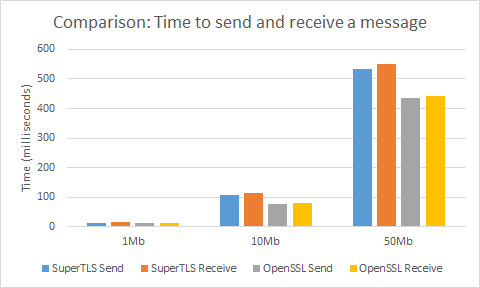
\includegraphics[width=9cm]{eval_time_2}
\centering
\caption{Comparison between the time it takes to send and receive a message using SuperTLS and OpenSSL 1.0.2g.}
\label{fig:eval_time_2}
\end{figure}

Figure \ref{fig:eval_time_2} shows the comparison between the time it takes to send, and receive, a message through a SuperTLS channel and the time it takes to send, and receive, the same message through an OpenSSL/TLS channel. Overall, a message sent through a SuperTLS channel takes, in average, 22,88\% longer than a message sent OpenSSL. For example, a 50 Megabytes message takes, in average, $534,55$ ms to be sent through a SuperTLS, while using OpenSSL, the same message takes $435,01$ ms to be sent.
The overhead generated by using multiple ciphers and signatures exists, as expected, but it is much smaller than the worst case.

In Section \ref{subsubsec:theretical-msg-size}, we already did an analysis of the expected message size increase, using variables. In order to validate the premise that the message increase is the same considering the same message size, we measured the increase in the message size, in bytes, comparing, once again, SuperTLS and OpenSSL channels.
A 100 Kilobytes plaintext message converts into a ciphertext of $102 771$ bytes long, using SuperTLS. Using OpenSSL, the same message corresponds to a ciphertext of $102 603$ bytes. Concluding, sending a 100 Kb message through SuperTLS costs an additional $168$ bytes. Although, as stated before, the number of extra bytes sent is not directly proportional to the message size. Assuming that they were directly proportional, sending a 1 Megabyte message through a SuperTLS channel would cost $172 032$ bytes.

We also evaluated the message size of the ciphertext of a 1 Megabyte plaintext message. A 1 Mb plaintext message corresponds to a ciphertext of $1 029 054$ bytes using SuperTLS, while using OpenSSL, the same message converts into a message of $1 025 856$ bytes. Concluding, sending 1 Mb through a SuperTLS channel costs an additional $3 198$ bytes than using a OpenSSL channel.
As we can conclude, the values are not definitely not directly proportional.

\subsection{Management and Cost}

SuperTLS is a communication channel which objective is to provide a vulnerability-tolerant channel, using diversity and redundancy, to provide security. Nevertheless, SuperTLS, such as TLS and other protocols, uses certificates and need to be managed.
A cloud or server using a TLS-based communication channels, such as OpenSSL, to communicate in a secure fashion with another cloud only needs one certificate. If the same cloud or server decides to use SuperTLS, it will need, at least $2$ certificates, and at maximum, $k$ certificates. Although certificates are not very expensive, they represent an annual cost to the cloud or server. If the cloud or server decides to use SuperTLS, it can be used with just one certificate, but diminishing the diversity and, consequently, the potential security increase.

Using a diversity factor $k = 2$, the cost of the certificates duplicates, which can be an issue for some cloud providers or companies. Nevertheless, it is our belief that the additional cost of having two certificates instead of one is compensated by the increase of security and vulnerability-tolerance provided by SuperTLS.

Regarding management, there is the need to manage two certificates instead of one. This does not represent a huge increase of management costs as the number of certificates only duplicates. If the cloud's owner decides to use SuperTLS with a diversity factor $k > 2$, the management costs of maintaining the $k$ certificates might represent an significant increase of management costs.

\section{Conclusions}

SuperTLS is a diverse and redundant vulnerability-tolerant secure communication channel designed for communication between clouds. It aims at increasing security using the most diverse cipher suites to tolerate vulnerabilities in any encryption mechanism used in the communication channel. We used a default diversity factor $k = 2$ for SuperTLS, and the preferred cipher suite to use with a SuperTLS are \textit{TLS\_ECDHE\_ECDSA\_WITH\_AES\_256\_GCM\_SHA384} + \\\textit{TLS\_RSA\_WITH\_AES\_128\_CBC\_SHA256}. In order to evaluate our solution, we compared it to an OpenSSL 1.0.2g communication channel. While expected to be $k, k = 2$ times slower than an OpenSSL channel, SuperTLS' evaluation demonstrated that using diversity and redundancy of cryptographic mechanisms does not generate the expected overhead. SuperTLS takes, in average, 22,88\% longer to send a message than TLS/OpenSSL, but considering the increase in security, this overhead is acceptable.

Overall, considering the additional costs of having an extra certificate, the time increase, and potential management costs, the SuperTLS is a very good communication channel for clouds to communicate, using diversity to mitigate vulnerabilities existent.

%\end{document}  % This is where a 'short' article might terminate

%ACKNOWLEDGMENTS are optional
%\section{Acknowledgments}
%This section is optional; it is a location for you
%to acknowledge grants, funding, editing assistance and
%what have you.  In the present case, for example, the
%authors would like to thank Gerald Murray of ACM for
%his help in codifying this \textit{Author's Guide}
%and the \textbf{.cls} and \textbf{.tex} files that it describes.

%\section{Future Work}
%
%\begin{itemize}
%\item{SuperTLS is based only on a version of OpenSSL. An interesting feature would be diversifying two different libraries and make them compatible with each other. This would increase diversity in the code and, optionally, programming languages. Also, different teams think differently and this could potentially lead to make SuperTLS to tolerate more vulnerabilities regarded with the implementation;}
%\item{Using SHA-3 for hash to increase diversity when it is supported by TLS}
%\item{SuperTLS performed rather well comparing with OpenSSL. The only existing approach other than SuperTLS is TLS-over-TLS. Future work: Compare SuperTLS with TLS-over-TLS.}
%\end{itemize}

%
% The following two commands are all you need in the
% initial runs of your .tex file to
% produce the bibliography for the citations in your paper.
\bibliographystyle{abbrv}
\bibliography{sigproc}  % sigproc.bib is the name of the Bibliography in this case
% You must have a proper ".bib" file
%  and remember to run:
% latex bibtex latex latex
% to resolve all references
%
% ACM needs 'a single self-contained file'!
%
%\section{References}
%Generated by bibtex from your ~.bib file.  Run latex,
%then bibtex, then latex twice (to resolve references)
%to create the ~.bbl file.  Insert that ~.bbl file into
%the .tex source file and comment out
%the command \texttt{{\char'134}thebibliography}.
% This next section command marks the start of
% Appendix B, and does not continue the present hierarchy
%\section{More Help for the Hardy}
%The sig-alternate.cls file itself is chock-full of succinct
%and helpful comments.  If you consider yourself a moderately
%experienced to expert user of \LaTeX, you may find reading
%it useful but please remember not to change it.
%\balancecolumns % GM June 2007
% That's all folks!
\end{document}
